
\begin{boxteo}Для абсолюно неперервного векторa $\begin{bmatrix}
	 \xi& \eta
	\end{bmatrix}^T$\\
$$\xi \independent \eta \Leftrightarrow f_{\xi, \eta} (x,y)= f_{\xi}(x) f_{\eta}(y) \quad \forall x,y \in \mathbb{R}$$
\end{boxteo}

\begin{proof}
$$
\begin{gathered}
1. \quad  F_{\xi, \eta} (x,y) = F_{\xi}(x) \cdot F_{\eta}(y) \Longrightarrow f_{\xi, \eta} (x,y) = f_{\xi}(x) \cdot f_{\eta}(y)\\
	2. \quad f_{\xi, \eta} (x,y) = f_{\xi}(x) \cdot f_{\eta}(y)\Longrightarrow F_{\xi, \eta} (x,y) = F_{\xi}(x) \cdot F_{\eta}(y)
\end{gathered}\quad \forall x,y \in \mathbb{R}
$$
2.
$$
F_{\xi, \eta} (x,y ) =  \int\limits_{-\infty}^{ x}{  \int\limits_{- \i}^{y}{ f_{\xi, \eta} (s,t) dsdt}} =  \int\limits_{- \i}^{ x}{  \int\limits_{-\i}^{y}{ f_{\xi} (s) \cdot f_{\eta} (t)dsdt}} =
$$
$$
= \int\limits_{-\i}^{ x}{ f_ \xi (s) ds}\cdot  \int\limits_{-\i}^{ +\infty}{f_\eta(t) dt} = F_{\xi}(s)\cdot F_{\eta}(t)
$$
1.
$$
f_{\xi, \eta} (x,y) = \frac{\partial^2 f}{\partial x \partial y} (x,y) = \frac{\d ^2}{\d x \d y} (F_{\xi}(x) \cdot F_{ \eta} (y) ) = \frac{\d}{\d x} (F_{\xi} (x) \cdot f_{\eta} (y) ) = f_{\xi}(x) \cdot f_{\eta}(y)
$$
\end{proof}

\subsection{Умовні розподіли та умовні математичні сподівання.}

\subsubsection{Дискретний вектор.}
$$
\begin{gathered}
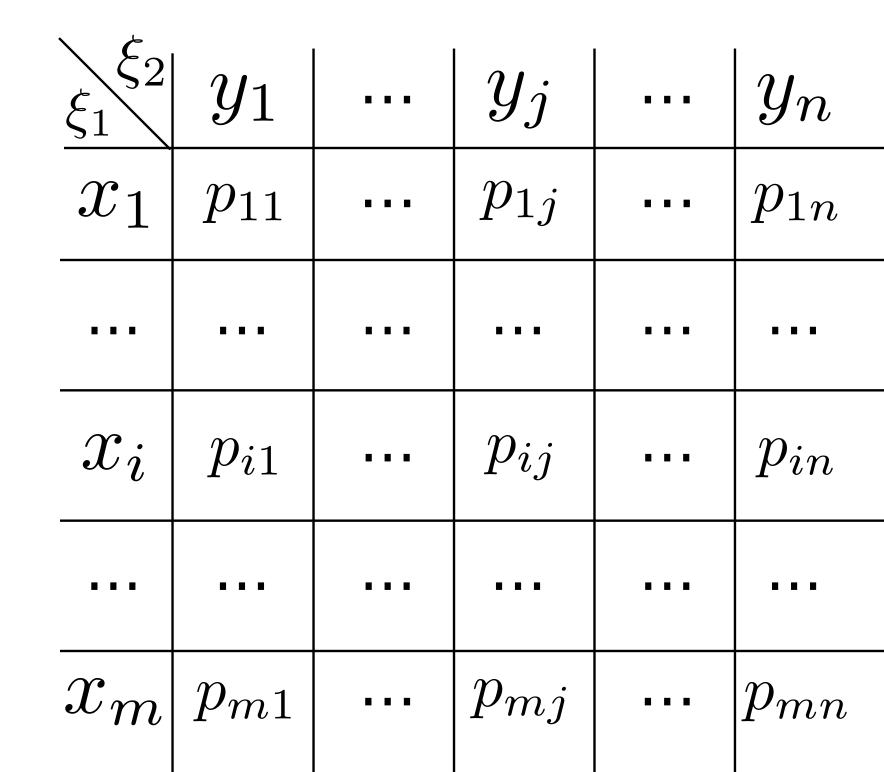
\includegraphics[scale=0.16]{images/14.png}
\end{gathered}\qquad\quad
\begin{gathered}
\text{Розподіли } \xi_2 \text{ за } \xi_1\\
\mathbb{P} \left\lbrace \xi_2 = y_j | \xi_2 = x_i \right\rbrace = \frac{\mathbb{P} \left\lbrace \xi_1 = x_i, \xi_2 = y_j \right\rbrace}{ \mathbb{P} \left\lbrace \xi_1 = x_i \right\rbrace} = \\
= \frac{p_{ij}}{  \sum\limits_{j = 1}^{n}{ p_ij}}
\end{gathered}
$$

\begin{center}
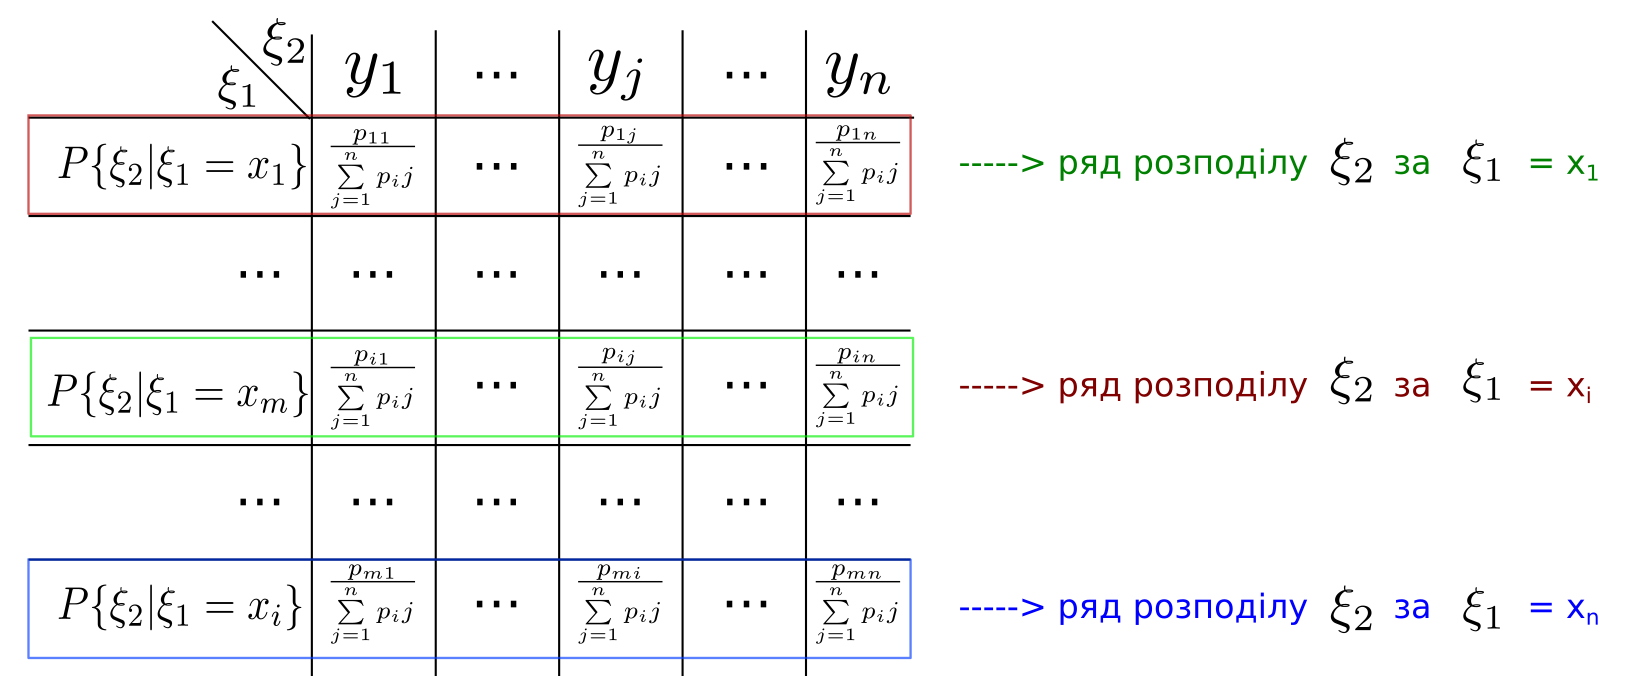
\includegraphics[scale=0.28]{images/20.png} \end{center}
$$
\mathbb{E}(\xi_2 | \xi_1 = x_i)  =  \sum\limits_{j = 1}^{ n}{ y_j \mathbb{P} \left\lbrace \xi_2 = y_j | \xi_1 = x_i \right\rbrace } =  \sum\limits_{j = 1}^{n}{ y_{j} \cdot \frac{p_{ij} }{  \sum\limits_{k = 1}^{ n}{p_{ik}}}}= \frac{  \sum\limits_{j = 1}^{ n}{ y_j p_{ij}}}{  \sum\limits_{j = 1}^{n}{ p_{ij}}}
$$
$$
\begin{matrix}
	\xi_1 & x_1 & \cdots  &x_i & \cdots & x_m \\
	\mathbb{E}_{\xi_2 | \xi_1=x_k}  &  \frac{  \sum\limits_{j = 1}^{ n}{ y_j p_{1j}}}{  \sum\limits_{j = 1}^{n}{ p_{1j}}}  & \cdots  &\frac{  \sum\limits_{j = 1}^{ n}{ y_j p_{ij}}}{  \sum\limits_{j = 1}^{n}{ p_{ij}}}  & \cdots & \frac{  \sum\limits_{j = 1}^{ n}{ y_j p_{mj}}}{  \sum\limits_{j = 1}^{n}{ p_{mj}}}  \\
	\mathbb{P} \left\lbrace \xi_1 = x_k \right\rbrace &   \sum\limits_{j = 1}^{n}{ p_{ij}} & \cdots  &\sum\limits_{j = 1}^{n}{ p_{ij}} & \cdots & \sum\limits_{j = 1}^{n}{ p_{mj}} \\
\end{matrix}
\begin{gathered}
\longrightarrow \text{ряд розподілу}\\
\mathbb{E}(\xi_2| \xi_1)
\end{gathered}
$$
$$
\mathbb{E}[ \mathbb{E} (\xi_2 | \xi_1)] =
\frac{  \sum\limits_{j = 1}^{n}  {y_j \cdot p_{1j}} }   {  \sum\limits_{j = 1}^{ n}{ p_{1j}}} \cdot  \sum\limits_{j = 1}^{ n}{ p_{1j}}+ ... +
\frac{  \sum\limits_{j = 1}^{n}{y_j \cdot p_{mj}} }   {  \sum\limits_{j = 1}^{ n}{ p_{mj}}} \cdot  \sum\limits_{j = 1}^{ n}{ p_{mj}} =  \sum\limits_{i = 1}^{m}{  \sum\limits_{j =1 }^{ n}{ y_j p_{ij}}} = \mathbb{E}\xi_2
$$
$$
\mathbb{E}[ \mathbb{E} (\xi_2 | \xi_1)] = \mathbb{E}  \xi_2  \quad \quad \quad \mathbb{E}[ \mathbb{E} (\xi_1 | \xi_2)] = \mathbb{E}  \xi_1
$$
\subsubsection{Абсолютно неперервний вектор.}
$$
\overline{\xi}  \begin{bmatrix}
 \xi_1 \\ \xi_2
\end{bmatrix} \qquad f_{\overline{\xi}} (x,y) - \text{ сумісна щільність розподілу.}
$$
$
f_{\xi_2 | \xi_1} (y|y) = f_{\xi_2| \xi_1 = x} (y)
$ - умовна щільність другої координати за першою.\\

$F_{\xi_2 | \xi_1 = x} (y)$ - умовна функція розподілу $\xi_2$ за умови $\xi_1 = x$.\\
$ F_{\xi_2 | \xi_1 = x} (y) = \mathbb{P} \left\lbrace \xi_2 < y | \xi_1 = x  \right\rbrace = \frac{\mathbb{P} \left\lbrace \xi_1  = x , \xi_2 < y \right\rbrace}{ \mathbb{P} \left\lbrace \xi_1 = x \right\rbrace} = \frac{0}{0} $
\\$$   F_{\xi_2 | \xi_1 = x} (y) = \lim\limits_{\varepsilon \to  \infty}{
 \mathbb{P} \left\lbrace  \xi_2 | \xi_1 \in [x, x+ \varepsilon ) \right\rbrace
 } =  \frac{ \mathbb{P} \left\lbrace \xi_1 \in [x, x+ \varepsilon ) , \xi_2 \in (- \i, y)\right\rbrace}{ \mathbb{P} \left\lbrace \xi_1 \in [x, x + \varepsilon ) \right\rbrace} =
  $$
	$$
	=  \lim\limits_{\varepsilon \to  0} { \frac{\int\limits_{x}^{ x+\varepsilon }{ ds  \int\limits_{- \i}^{ y}{ f_{ \overline{\xi}}}(s,t)dt}}{
  \int\limits_{x}^{ x+\varepsilon }{ f_{\xi_1} (s) ds}}
  } =    \lim\limits_{\varepsilon \to  0} { \frac{\varepsilon \cdot\int\limits_{x}^{ x+\varepsilon }{ ds  \int\limits_{- \i}^{ y}{ f_{ \overline{\xi}}}(s,t)dt}}{ \varepsilon \cdot
  \int\limits_{x}^{ x+\varepsilon }{  f_{\xi_1} (s) ds}}
  }  =  \fbox{$ \displaystyle\frac{  \int\limits_{- \i}^{ y}{ f_{ \overline{\xi}} }(x,t)dt}{ f_{\xi_1} (x)} = F_{\xi_2 | \xi_1 = x} (y)$}
	$$
Знаючи умовну функцію розподілу, можемо знайти умовну щільність:
	$$
	f_{\xi_2 | \xi_1 = x} = F_{\xi_2| \xi_1 = x}'(y) = \frac{f_{\overline{\xi}}(x,y)}{ f_{\xi_1}(x)}
	$$
Знайдемо умовне математичне сподівання $\xi_2$ за $\xi_1$
	$$
	\mathbb{E}(\xi_2 | \xi_1 = x) =  \int\limits_{-\i}^{ +\infty}{ y \cdot f_{\xi_2 | \xi_1 = x} dy} =  \int\limits_{-\i}^{ +\infty}{ y \cdot \frac{f_{\overline{\xi}}(x,y)}{ f_{\xi_1} (x)}  dy} =
	\frac{
	\int\limits_{-\i}^{ +\infty}{ y \cdot f_{\overline{\xi}}(x,y)}dy}{ f_{\xi_1} (x)}
	$$
$ \mathbb{E} (\xi_2| \xi_1)$ - випадкова величина, яка спочатку визначає, куди попала умова (чому дорівнює $x \longleftarrow \xi_1$), а далі визначає $\mathbb{E}(\xi_2| \xi_1 = x)$.\\
$\mathbb{E}(\xi_2| \xi_1)$ - набуває значення $ \mathbb{E}(\xi_2 | \xi_1 = x)$, коли $\xi_1$ набула значення $x$.
$$\xi_1 \longrightarrow x \Rightarrow \mathbb{E}(\xi_2 | \xi_1) \longrightarrow \mathbb{E}(\xi_2 | \xi_1 = x)$$
$ \mathbb{E}(\xi_2 | \xi_1)$ є функцією від $\xi_1$. Якою? $ \mathbb{E}(\xi_2 | \xi_1 = x)$\\
$ \mathbb{E} (\xi_2 | \xi_1 ) = \Psi (\xi_1)$, де $ \Psi(x) = \mathbb{E}( \xi_2 | \xi_1 = x)$

\begin{center}
	Формула повного математичного сподівання (?$\mathbb{E}[\mathbb{E}(\xi_2 | \xi_1)] = \mathbb{E}\xi_2$?)
\end{center}
$$\mathbb{E}[\mathbb{E}(\xi_2 | \xi_1)] = \mathbb{E}\Psi  (\xi_2) =  \int\limits_{-\i}^{ +\infty}{\Psi(x) \cdot f_{\xi_1} (x)dx} =  \int\limits_{-\i}^{ +\infty}{
\frac{
\int\limits_{-\i}^{ +\infty}{ y \cdot f_{\overline{\xi}}(x,y)}dy}{ f_{\xi_1} (x)} \cdot f_{\xi_1} (x) dx} = \mathbb{E} \xi_2$$

\section{Характеристичні функції.}

$\xi$ - випадкова величина. Загальна характеристика такої величини - функція розподілу. Існує для кожної величинию. Також є характеристики, такі як ряд розподілу та щільність розподілу - існують не завжди. Введемо ще одну характеристику, яка буде існувати для будь-якої випадкової величини.\\
\bd
\textbf{Характеристична функція випадкової величини.}
$$
\chi_ \xi (t) = \mathbb{E}(\cos{(t \xi)} + i \sin{(t \xi)}   ) =  \mathbb{E}( e^{ it \xi})
$$
\begin{center}
	\fbox{$ X_ \xi : \mathbb{R} \rightarrow \mathbb{C}$}
\end{center}
\ed
Як шукати? Дискретний випадок: $  \sum\limits_{i = 1}^{ n(\infty)}{ e^{itx_i}p_i}$\\
Для абсолютно неперервної величини: $  \int\limits_{-\i}^{ +\infty}{ e^{itx}f_ \xi (x)dx}$

\subsection{Властивості характеристичних функцій.}

$\xi$ - випадкова величина. $\chi_ \xi(t) = \mathbb{E} e^{et \xi} =  \int\limits_{-\i}^{ +\infty}{ e^itx f_{\xi}(x)dx}$\\

1. Характеристична функція є унікальною характеристикою ймовірнісного розподілу.\\
2. $ \chi_{\xi} (0) = 1  \qquad \chi_{\xi} (0) =  \mathbb{E} e^0 = 1$.\\
3. $	\left| \chi_ \xi (t)\right| \leq 1 \quad \forall t \in \mathbb{R}$
$$
\left| \mathbb{E} e^{it \xi} \right| = \left| \mathbb{E}\cos{(t \xi)} + i \mathbb{E} \sin{(t \xi)}   \right| = \sqrt{
\mathbb{E} \cos{(t \xi)}^2 + \mathbb{E} \sin{(t \xi)}^2
}  = 1
$$
4. $\chi_ \xi$ - неперервна за $t$ для $\xi$ - абсолютно неперервна випадкова величина.
$$
\chi_ {\xi} (t) =  \int\limits_{-\i}^{ +\infty}{ e^{itx} f_{\xi} (x) dx}
\quad \longleftarrow \quad
\chi_ {\xi} (t+h) =  \int\limits_{-\i}^{ +\infty}{ e^{i(t+h)x} f_{\xi} (x) dx}
$$
$$
(\chi_{\xi} - \text{ непервна в т. } t ) \Longleftrightarrow  \lim\limits_{h\to0}{ \chi_ \xi (t+h) } = \chi_{\xi} (t)
$$
Для $
 \lim\limits_{h\to  0}{  \int\limits_{-\i}^{ +\infty}{ e^{i(t+h)x} f_{\xi}(x)}dx} =  \int\limits_{-\i}^{ +\infty}{ e^{itx} f_ \xi(x) dx}
$, треба щоб $  \int\limits_{ -\i}^{ +\infty}{e^{itx}f_ \xi (x)dx}$ збігався рівномірно на $t \in \mathbb{R}$. $ \left| e^{itx} \cdot f_{\xi}(x) \right| = \left| f_{\xi}(x) \right| = f_{\xi}(x) = M(x) $- мажорантний ряд.\\
$$
 \int\limits_{-\i}^{ +\infty}{ M(x) dx } =  \int\limits_{-\i}^{ +\infty}{f_{\xi}(x)dx } = 1 < \i
$$
$
 \int\limits_{-\i}^{ +\infty}{ e^{itx} f_{\xi} (x) dx }
$ - збігається рівномірно за озн. Вейерштрасса.\\
5. $ \xi_1 \independent \xi_2 \Longrightarrow \chi_{\xi_1 + \xi_2} (t) = \chi_ {\xi_1} (t) \cdot  \chi_ {\xi_2} (t) $\\
6. Якщо $ \exists \mathbb{E} \xi^n$, то $\mathbb{E} \xi^n = \frac{1}{i^n}\cdot \chi^{(n)}_ \xi (0) $.
\begin{proof} В неперервному випадку.
$$
\mathbb{E} \xi^n =  \int\limits_{-\i}^{ +\infty}{x^n \cdot f_ {\xi} (x)dx}
$$
$$
\chi (t) = \mathbb{E} e^{it \xi} =  \int\limits_{-\i}^{ +\infty}{ e^{itx} f_ \xi(x) dx}
$$
$$
\chi^{(n)}(t) =  \int\limits_{-\i}^{ +\infty}{ (ix)^n e^{itx} f_ \xi  (x) dx}
$$
Але потрібна рівномірна збіжність. Скористаємося озн. Вейерштрасса:
$$
\left| (ix)^n e^{itx} f_ \xi  (x)  \right| = \left| x \right|^n \cdot f_ \xi (x) = M(x):
$$
$$
 \int\limits_{-\i}^{ +\infty}{ M(x)dx} =  \int\limits_{-\i}^{ +\infty}{ \left| x \right|^n \cdot f_{\xi}(x)dx < \i }
$$
$$
\chi^{(n)}(0) = i^n  \int\limits_{-\i}^{ +\infty}{ x^n \cdot f_{\xi} (x)dx} = i^n \cdot \mathbb{E}(\xi^n)
$$

\end{proof}
$6^*. $ Якщо існує $ \exists \chi (t)^{(n)}$, то виконується попередня властивість. $(n - \text{ парне.})$\\

7. $\chi_{a \xi +b} (t) = \mathbb{E} e^{i(a \xi + b)t}  = \mathbb{E} ( e^{ ia \xi t} \cdot e^{ibt}) = e^{ibt} \cdot \mathbb{E} e^{ai \xi t} = e^{ibt} \chi_{\xi} (at) $\\
8. $\chi_{-\xi}(t) = \chi_{\xi} (-t) = \mathbb{E} e^{i(-\xi)t} =  \overline{ \mathbb{E} e^{i \xi t}} = \overline{\chi_{\xi} (t)}$\\
9. Нехай випадкова величина $\xi$ має симетричний розподіл.
$$
\mathbb{P} \left\lbrace \xi \in B \right\rbrace = \mathbb{P} \left\lbrace \xi\in -B \right\rbrace \Leftrightarrow \begin{cases}
\xi - \text{ ДВВ: Ряд розподілу симетричний відносно 0.} \\
 \xi - \text{ АНВВ: } f_{\xi}(x) = f_{\xi}(-x)
\end{cases}
$$

\def\char{\chi_{\xi}}
Тоді: $- \xi \equiv \xi  \Longrightarrow \overline{\char(t)} = \char(t) = \char(-t)$.\\
Це означає, що $\char (t)$ - парна, дійсного значення.\\
10. Нехай $\xi$ не є обов'язково симетричною. Тоді $\overline{\char(t)} = \chi_{-\xi}(t) = \char(-t)$. \\Інакше, парність $\char (t)$ означає її дійснозначність.
\newpage
\subsection{Основні ''проблеми'' характеристичних функцій.}
1. За функцією $\chi$ досить важко визначити, чи є вона характеристичною функцією деякої випадкової величини.\\
2. Якщо $\chi$ - дійсно характеристична функція деякої випадкової величини, то важко зрозуміти, чи буде $\xi$ ДВВ або АНВВ.\\

Задача: Чи є функція характеристичною? Якщо є, то для якого розподілу?\\
Основні критерії, яким має відповідати характеристична функція - це 4 властивості наведені нижче. Якщо одна з властивостей не виконується, то функція не є характеристичною. Інакше, потрібно навести конкретний розподіл, який описує задана функція.\\
1. $\chi(0) = 1$\\
2. $ \left| \chi(t) \right| \leq 1 	$\\
3. Неперервна і визначена $\forall t \in \mathbb{R}$.\\
4. $\chi (t) \in \mathbb{R} \quad \forall t \in \mathbb{R} \Longleftrightarrow
\chi(-t) = \chi (t)
$\\

\subsection{Характеристичні функції головних ймовірнісних розподілів.}
\subsubsection{Дискретні розподіли.}
З дискретними розподілами працювати легше. В загальному випадку, величина приймає невід'ємні цілі значення. Раніше вводили поняття генератрисси:
$$
G_{\xi}(z) =  \sum\limits_{k = 0}^{ \infty}{ p_k \cdot z^k}
$$
В данному розділі розглядаємо пов'язану функцію функцію:
$$
\char (t) =   \sum\limits_{k = 0}^{ \infty}{p_k \cdot e^{itk}} =  \sum\limits_{k = 0}^{ \infty}{ p_k \cdot (e^{it})^k} = G_{\xi}(e^{it})
$$

$$\begin{matrix}
	\xi \sim Bin(n,p) & \Longrightarrow & G_{\xi}(z) = (pz + q)^n  & \Longrightarrow& \char (t) = (pe^{it} + q)^n\\
	\xi \sim Geom_{0}(p) & \Longrightarrow & G_{\xi}(z) = \frac{p}{1-qz} & \Longrightarrow& \char (t)  = \frac{p}{1 - qe^{it}}\\
		\xi \sim Geom_{1}(p) & \Longrightarrow & G_{\xi}(z) = \frac{pz}{1-qz} & \Longrightarrow& \char (t)  = \frac{pe^{it}}{1 - qe^{it}}\\
		\xi \sim Pois(\lambda)& \Longrightarrow & G_{\xi}(z) = e^{\lambda(z-1)}& \Longrightarrow & \char (t)  =  e^{\lambda (e^{it} -1)}\\
		% \xi \sim & \Longrightarrow & G_{\xi}(z) =& \Longrightarrow & \char (t)  = \\
\end{matrix}
$$
Таким чином, ми бачимо, що характеристичні функції напряму пов'язані з генератриссами. При роботі з ДВВ зручніше працювати з генератриссами, але на відміну від генератрисс, хактеристична функція визначена для всіх видів випадкових величин. Перейдемо до абсолютно неперервного випадку.

\subsubsection{Абсолютно неперервні розподіли.}
Згадаємо: $ \char (t) =  \int\limits_{-\i}^{ +\infty}{ e^{itx} f_{\xi}(x) dx}$
$$
\xi \sim \mathbf{U(a,b)}. \qquad \char (t) = \int\limits_{-\i}^{ +\infty}{ e^{itx} \begin{cases}
	\frac{1}{b-a}, & x\in [a,b];\\
	0, & x \notin [a,b];
\end{cases}} = \frac{1}{a-b}  \int\limits_{a}^{ b}{ e^{itx}dx}  =  \frac{e^{itb} - e^{ita}}{ it (b-a)}
$$

$$
\chi_{U(-a,a)}(t) = \begin{cases}
	\frac{e^{ita} - e^{-ita}}{2iat}, & t \neq 0;\\
	1, & t = 0;
\end{cases}= \begin{cases}
	\frac{\sin{(at)} }{at}, & t \neq 0;\\
	1, & t = 0;
\end{cases}
$$

$$
\xi \sim \mathbf{Exp(\lambda)}. \qquad \char (t) =  \int\limits_{0}^{ +\infty}{ \lambda \cdot e^{-\lambda x}e^{itx}dx} = \frac{\lambda}{it- \lambda} e^{x(it- \lambda	)} \Bigg|_{x=0}^{+\i}= \frac{\lambda}{ \lambda - it}
$$
Для гаусівського розподілу: спочатку розглянемо $\xi_0 \sim N(0,1).$ Потім скористаємося властивістю $\xi =  a+ \sigma \xi_0$, де $\xi \sim N(a, \sigma^2)$.
$$
\xi \sim \mathbf{N(0, 1)}. \qquad \chi_{\xi_0} (t) = \mathbb{E} e^{it \xi} =  \int\limits_{-\i}^{ +\infty}{ e^{itx} } = \frac{1}{\sqrt{2\pi}}  \int\limits_{-\i}^{ +\infty}{ e^{itx}\cdot e^{- \frac{x^2}{2} }}dx =
$$
$$
= \left|  \begin{gathered}
u = e^{- \frac{x^2}{2}} \\
dv = e^{itx}dx
\end{gathered} \quad \begin{gathered}
du =  -x \cdot e^{- \frac{x^2}{2}} \\
v =  \frac{1}{it} e^{itx}
\end{gathered}\right| = \frac{1}{\sqrt{2\pi}} \left( \frac{1}{it} \cdot e^{itx} e^{- \frac{x^2}{2} } \Bigg|_{-\i}^{+\i}  + \frac{1}{it}  \int\limits_{-\i}^{ +\infty}{ e^{itx} x e^{- \frac{x^2}{2} }dx}  \right)  =
$$
$$
= \frac{1}{\sqrt{2\pi}}\frac{1}{it}  \int\limits_{-\i}^{ +\infty}{ e^{itx} x e^{- \frac{x^2}{2} }dx} = \chi_{\xi_0} (t)
$$

$$
\chi_{\xi_0}'(t) = \frac{1}{2\pi}  \int\limits_{-\i}^{ +\infty}{ ix e^{itx} e^{- \frac{x^2}{2} }dx}  \quad \Longrightarrow \quad \chi_{\xi_0}'(t) = -t\chi_{\xi_0}(t)
$$
$$
\frac{d \chi}{ dt} = -t \chi \qquad  \int\limits_{}^{}{ \frac{d \chi}{\chi} } = -  \int\limits_{}^{}{ tdt} \qquad \ln{ \left| \chi  \right|  = - \frac{t^2}{2}  + C } \qquad \chi(t) = K \cdot e^{ - \frac{t^2}{2} }
$$
$$
\chi (0) = 1 = K \quad  \Longrightarrow \quad \fbox{$ \chi_{\xi_0} (t) = \chi_{N(0,1)}(t) = e^{- \frac{t^2}{2} } $}
$$
\begin{center}
\fbox{$ \chi_{N(a, \sigma^2)} (t) = e^{iat - \frac{\sigma^2 t^2}{2} } $}
\end{center}
\vfill

\subsection{Ймовірнісні розподіли, стійкі відносно додавання.}

\begin{defo}
	Розподіл називають стійким відносно додавання, якщо сума двох незалежних випадкових
	величин, що мають цей розподіл (можливо, з різними параметрами), також має цей розподіл.
\end{defo}
$Pois(\lambda)$ - стійкий розподіл. Це означає, що:


$$
\independent
\begin{cases}
	\xi_1 \sim Pois(\lambda_1)\\
	\xi_2 \sim Pois(\lambda_2)
\end{cases} \Longrightarrow \xi_1 + \xi_2 \sim Pois(\lambda_1 + \lambda_2)
$$


Доведемо задопомогою характеристичної функції розподілу:

$$
\begin{cases}
\chi_{\xi_1} (t) = e^{\lambda_1(e^{it} - 1)} \\
\chi_{\xi_2} (t) = e^{\lambda_2(e^{it} - 1)} \\
\end{cases} \Longrightarrow \chi_{\xi_1 + \xi_2} (t) = \chi_{\xi_1} (t)\cdot \chi_{\xi_2} (t)= e^{(\lambda_1 + \lambda_2)( e^{it} -1 ) }
$$
Остаточно: \fbox{$ \xi_1 + \xi_2 \sim Pois(\lambda_1 + \lambda_2)$}\\

$ N(a, \sigma^2)$ - стійкий розподіл.
$$
\independent
\begin{dcases}
	\xi_1 \sim  N(a_1, \sigma_1^2)\\
	\xi_2 \sim  N(a_2, \sigma_2^2)
\end{dcases} \qquad
\begin{dcases}
\chi_{\xi_1}  = e^{ia_1 t - \frac{\sigma_1^2 t^2 }{2} } \\
\chi_{\xi_2}  = e^{ia_2 t - \frac{\sigma_2^2 t^2 }{2} }
\end{dcases}$$
$$
\chi_{\xi_1 + \xi_2 }(t)  = \chi_{\xi_1} \cdot \chi_{\xi_2} (t)= e^{i(a_1+ a_2) t - \frac{(\sigma_1+ \sigma_2)^2 t^2 }{2} }= \chi_{N(a_1+a_2, \sigma_1^2 + \sigma_2^2)} (t)
$$
Остаточно: \fbox{$
\xi_1 + \xi_2 \sim N(a_1+a_2, \sigma_1^2 + \sigma_2^2)
$}\\
   \\
Розглянемо біноміальний розподіл:\quad
$Bin(n, p)$
$$ \qquad \independent
\begin{dcases}
	\xi_1 \sim  Bin(n_1, p)\\
	\xi_2 \sim  Bin(n_2, p)
\end{dcases}  \qquad \begin{dcases}
\chi_{\xi_1} (t) = \left( pe^{it} + q \right)^{n_1}\\
	\chi_{\xi_2} (t) = \left( pe^{it} + q \right)^{n_2}
\end{dcases}$$
$$
\chi_{\xi_1 + \xi_2} (t) = \left( pe^{it} + q \right)^{n_1} \cdot \left( pe^{it} + q \right)^{n_2} = \left( pe^{it} + q \right)^{n_1 + n_2}
$$
Остаточно: \fbox{$
\xi_1 + \xi_2 \sim Bin(n_1 + n_2, p)
$}
\\
   \\
Задача: знайти щільність розподілу $f_{\xi}(x)$ за харатеристичною функцією.\\
$$
\char (t) =  \int\limits_{-\i}^{ +\infty}{ e^{itx} f_{\xi}(x)dx} - \text{перетворення Фур'є} \qquad f\xrightarrow{F}\chi
$$
$$
f_{\xi}(t) =  \frac{1}{2\pi} \int\limits_{-\i}^{ +\infty}{ e^{itx} \chi_{\xi}(x)dx} - \text{обернене перетворення} \qquad \chi \xrightarrow{F}f
$$

\newpage

\subsection{Характеристичні функції випадкових векторів.}
\def\xx{\chi_{\overline{\xi}}}
\subsubsection{Означення.}
Розглядаємо випадковий вектор $
\overline{\xi}= \begin{bmatrix}
 \xi_1 \\
 \vdots\\
 \xi_n
\end{bmatrix}
$ . Характеристична функція:

$$
\xx (\overline{t}) = \xx (t_1, t_2, ..., t_n) = \mathbb{E} e^{i< \overline{\xi}, \overline{t}>}  = \mathbb{E} e^{i  \left( t_1 \xi_1 + ... + t_n \xi_n \right) }
$$
Для дискретного випадкового вектора $\overline{\xi}$:
$$
\xx (\overline{t}) =  \sum\limits_{i_1 = 1}^{ m_1}\cdots  \sum\limits_{i_n = 1}^{ m_n}{
e^{i \left( t_1 x_1^{(i_1)}+ ... + t_n x_n^{(i_n)} \right) } \cdot \mathbb{P} \left\lbrace \xi_1 = x^{(i_1)}, ..., \xi_n = x_n^{(i_n)} \right\rbrace
}
$$
Для абсолютно неперервного випадкового вектора $\overline{\xi}$:
$$
\xx (\overline{t}) =  \begin{gathered}
   \\
	 \int \cdots  \int \\
	 {\small \mathbb{R}^{n}}
\end{gathered} e^{i(t_1 x_1 + ... + t_n x_n)} f_{\overline{\xi}}(x_1, ... , x_n)dx_1...dx_n
$$

\subsubsection{Властивості характеристичної функції випадкового вектора.}
1. $\xx $ - унікальна характеристика випадкового вектора. Проте, за однакової характеристичної функції неможна вважати, що вектори однакові. Можна вважати, що вони мають однакові розподіли. Наведемо приклад:
$$
\xi \sim U(-1, 1) \qquad - \xi \sim U(-1, 1) \qquad \xi \neq - \xi \qquad \xi \circeq -\xi
$$
2. $\xx (\vec{0}) = 1$\\
3. $ \left| \xx (\overline{t}) \right| \leq 1 $\\
4. $\xx \in C(\mathbb{R}^n)$\\
5. Якщо $ \overline{\xi_1 } \independent \overline{\xi_2} \Longrightarrow
\chi_{\overline{\xi_1} + \overline{\xi_2}} (t) = \chi_{\overline{\xi_1}} (t) \cdot \chi_{\overline{\xi_2}} (t)$\\
6. $ \exists \mathbb{E} \left( \xi_1^{k_1}\cdot ... \cdot \xi_n^{k_n} \right)   \Longrightarrow
\mathbb{E} \left( \xi_1^{k_1}\cdot ... \cdot \xi_n^{k_n} \right)   =
\dfrac{1}{ i^{k_1 + ... + k_n}} \cdot
\dfrac{\partial^{ k_1 + ... + k_n}}{\partial t_1^{k_1} \cdot ...\cdot \partial t_n^{k_n}} \xx (\vec{0})  $\\
7. $ \chi_{A \overline{\xi} + \overline{b}} (\overline{t}) = \mathbb{E} e^{ i <A \overline{\xi} + \overline{b}, \overline{t}>} =
 \mathbb{E}  \left( e^{ i <A \overline{\xi}, \overline{t}>} \cdot e^{ i <\overline{b}, \overline{t}>} \right) =
 e^{ i <\overline{b}, \overline{t}>}  \mathbb{E}  e^{ i <\overline{\xi}, A^T \overline{t}>}  =
 e^{ i <\overline{b}, \overline{t}>}  \chi_{\overline{\xi}} \left( A^T \overline{t} \right)
	$\\
	8. Якщо координати вектора $\overline{\xi}$ - незалежні, Тоді: $
	\xx (\overline{t}) = \mathbb{E} e^{i ( t_1 \xi_1 + ... + t_n \xi_n)} =$ \\$ =
	\mathbb{E} \left( e^{it_1 \xi_1 }\cdot ... \cdot e^{it_n \xi_n } \right)  = \left( \mathbb{E} e^{it_1 \xi_1 } \right) \cdot ... \cdot \left( \mathbb{E} e^{it_n \xi_n } \right) = \chi_{\xi_1} (t_1) \cdot ... \cdot \chi_{\xi_n}(t_n)
	$\\
	Якщо координати незалежні, то характеристична функція розпадається на добуток маргінальних характеристичних функція. До речі, справедливе і оберненне твердження. Звідси, отримали критерій незалежності координат.
	\def\Laplas{\text{Ф}}
	\subsection{Гаусівські випадкові вектори.}
	$$ n= 1 \qquad \xi \sim N(a, \sigma^2)  \qquad f_{\xi} ( x)  = \frac{1}{\sigma\sqrt{2\pi} } e^{- \frac{(x-a)^2}{2\sigma^2} }  \qquad F_{\xi} (x) = \frac{1}{2}  + \Laplas \left( \frac{x-a}{\sigma}  \right)  $$

	$$
\sigma^2 = \mathbb{D} \xi \qquad a = \mathbb{E} \xi  \qquad \chi_{\xi} (t) = e^{iat - \frac{\sigma^2 t^2}{2} }
	$$
\subsubsection{Характеристики стандартного гаусівського розподілу.}

Нехай маємо стандартний гаусівський n-вимірний випадковий вектор:\\
$
\overline{\xi} = \begin{bmatrix}
 \xi_1 \\
 \vdots\\
 \xi_n
\end{bmatrix}
$, де $\xi_1, ..., \xi_n$ - незалежні $N(0,1) \Longrightarrow \overline{\xi} \sim N(\vec{0}, I)$.
$$
\mathbb{E} \overline{\xi} = \begin{bmatrix}
 \mathbb{E}\xi_1 \\
 \vdots\\
 \mathbb{E} \xi_n
\end{bmatrix} = \vec{0} \qquad \quad C_{ \overline{\xi}} = \begin{bmatrix}
 \mathbb{D} \xi_1 & cov(\xi_1, \xi_2) & \cdots & cov(\xi_1, \xi_n) \\
 cov(\xi_2, \xi_1) & \mathbb{D}\xi_2 & \cdots & cov(\xi_2, \xi_n)\\
 \vdots & \vdots & \ddots & \vdots\\
 cov(\xi_n, \xi_1)& cov(\xi_n, \xi_1) & \cdots & \mathbb{D}\xi_n
\end{bmatrix} = I^{n\times n}
$$
Для одновимірної стандартної величини $\xi \sim N(0,1)$:
$$
f_{\xi} (x) = \frac{1}{\sqrt{2\pi}}  e^{- \frac{x^2}{2} } \qquad F_{\xi} (x) = \frac{1}{2} + \Laplas(x) \qquad \chi_{\xi} (t) = e^{- \frac{t^2}{2} }
$$
Для стандартного вектора $\overline{\xi} \sim N(\vec{0}, I) \quad \overline{\xi} = \begin{bmatrix}
 \xi_1\\
 \vdots\\
 \xi_n
\end{bmatrix}$.
$$
f_{\overline{\xi}}(x_1, ..., x_n) = f_{\xi_1} (x_1) \cdot ... \cdot f_{\xi_n}(x_n) = \prod\limits_{j=1}^{n} \frac{1}{\sqrt{2\pi}} e^{ - \frac{x^2_j}{2} } =
 \frac{1}{(2\pi)^{ \frac{n}{2} }} e^{- \frac{ x^2_1 + ... + x^2_m}{2} } =
  \frac{1}{(2\pi)^{ \frac{n}{2} }} e^{- \frac{<\overline{x}, \overline{x}>}{2} }
$$

$$
F_{\overline{\xi}} (x_1, ... , x_n) = F_{\xi_1} (x_1) \cdot ... \cdot F_{\xi_n}(x_n) =  \prod\limits_{j=1}^{n} \left( \frac{1}{2} + \Laplas(x_j)  \right)
$$
$$
\chi_{t_1, ..., t_n} = \chi_{\xi_1} (t_1) \cdot ... \cdot \chi_{\xi_n} (t_n) = e^{- \frac{t_1^2}{2} \cdot ... \cdot \frac{t_n^2}{2}  } = e^{- \frac{t^2_1 + ... t^2_n}{2} 	} = e^{ - \frac{< \overline{t}, \overline{t}>}{2} }
$$

\subsubsection{Характеристика загального гаусівського розподілу.}
\def\veta{\overline{\eta}}
\def\vxi{\overline{\xi}}
Якщо $C$ - симетрична невід'ємно визначена матриця, то в неї існує квадратний корінь: така матриця $A: \quad A^2 = C.$\\
Розглянемо загальний гаусівський вектор: $\overline{\xi} \sim N(\vec{0}, I) $.\\ \quad \fbox{$\overline{\eta} = \overline{a} + A \overline{\xi}$} -  за означенням будемо називати гаусівським, тобто $\overline{\eta} \sim N(\overline{a}, C)$.\\
$$\mathbb{E}\veta = \mathbb{E} \left(  \overline{a} + A \overline{\xi}
 \right) = \mathbb{E} \overline{a} + \mathbb{E} \left( A \overline{\xi} \right) = \overline{a} + A \cdot \mathbb{E} \overline{\xi} = \overline{a}$$
 $$
 C_{\veta} = \mathbb{E}( \veta - \mathbb{E} \veta)( \veta - \mathbb{E} \veta)^T = \mathbb{E}( \overline{a} + A \overline{\xi} - \overline{a})( \overline{a} + A \overline{\xi} - \overline{a})^T =
 $$
 $$
 =\mathbb{E}( A \vxi \vxi^T A^T) = A \cdot \mathbb{E} \left( \vxi \vxi^T \right) \cdot A^T = A \cdot C_{\vxi} \cdot A^T = A \cdot I \cdot A^T = A^2 = C
 $$

Характеристична функція загального гаусівського вектора:\\
$$
\veta = \overline{a}+ A \vxi \text{ ,де }
A^2 = AA^T = C, \overline{\xi} - N(\vec{0}, I)$$
$$
\chi_{\veta} ( \overline{t}) = \chi_{A\vxi + \overline{a}} (\overline{t}) = e^{i <\overline{a}, \overline{t}>} \cdot \chi_{\vxi} \left( A^T \overline{t} \right) =
e^{i <\overline{a}, \overline{t}>} \cdot e^{- \frac{<A^T \overline{t}, A^T \overline{t}>}{2} } = e^{i <\overline{a}, \overline{t}> - \frac{<C \overline{t}, \overline{t}>}{2}  }
$$
Щільність розподілу вектора $\veta  \sim N( \overline{a}, C)$:\\
\textbf{Лема.} Щільність розподілу афінного перетворення. \\
Нехай маємо $\vxi$ - абсолютно неперервний випадковий вектор зі щільністю $f_{\vxi} (\overline{x})$. Маємо його афінне перетворення: $\veta = A\vxi + \overline{a}$(А - невироджена матриця).  Тоді, $\veta$ - абсолютно неперервний випадковий вектор зі щільністью $f_{\veta} (\overline{y})$:
$$
f_{\veta} (\overline{y}) = \frac{1}{ \left| \det(A) \right| }  f_ {\vxi} ( A^{-1}( \overline{y} - \overline{a}) )
$$

\begin{proof} Нехай $B \subset \mathbb{R}^n. \left( \text{Позначимо n-кратний інтеграл за множ. } B -  \iint\limits_{B} \right) $:
$$
  \iint\limits_{B} f_{\veta} (\overline{y})d \overline{y}=\mathbb{P} \left\lbrace \veta \in B \right\rbrace = \mathbb{P} \left\lbrace  A \vxi + \overline{a} \in B \right\rbrace = \mathbb{P} \left\lbrace  A \vxi \in B - \overline{a} \right\rbrace =
$$
$$
 = \mathbb{P} \left\lbrace \vxi \in A^{-1} \left( B - \overline{a} \right)  \right\rbrace = \iint\limits_{A^{-1} \left( B - \overline{a} \right) } f_{\overline{\xi}} ( \overline{\xi}) d \overline{\xi} = \left| \begin{gathered}
  \overline{y} = A \overline{x} + \overline{a}\\
	\overline{x}=  A^{-1} (\overline{y} - \overline{a})\\
	J = \left| \det (A^{-1}) \right|
 \end{gathered} \right| =
$$
$$
= \int\limits_{B}{ f_ {\vxi} ( A^{-1}( \overline{y} - \overline{a}) )  \left| \det (A^{-1}) \right| d \overline{y}  } =  \int\limits_{B}{ \frac{1}{ \left| \det(A) \right| }  f_ {\vxi} ( A^{-1}( \overline{y} - \overline{a}) ) d \overline{y}  }
$$
Інакше кажучи, інтеграли за будь-якою множиною збігаються т.т.т.к. збігаються підінтегральні функції. Приходимо до:
$$
  \iint\limits_{B} f_{\veta} (\overline{y})d \overline{y}= \int\limits_{B}{ \frac{1}{ \left| \det(A) \right| }  f_ {\vxi} ( A^{-1}( \overline{y} - \overline{a}) ) d \overline{y}  } \Longleftrightarrow   \fbox{$f_{\veta} (\overline{y}) = \frac{1}{ \left| \det(A) \right| }  f_ {\vxi} ( A^{-1}( \overline{y} - \overline{a}) ) $}
$$
\end{proof}

Повернемося до щільності розподілу загального вектора:
$$
f_{\veta} (\overline{x} )  = \frac{1}{ \left| \det{A} \right|  } f_{\vxi} (A^{-1} (\overline{x} - \overline{a})) = \frac{1}{ \left| \det{A} \right|  } \cdot \frac{1}{(2\pi)^{ \frac{n}{2} }} e^{- \frac{<A^{-1}(\overline{x} - \overline{a}), A^{-1}(\overline{x} - \overline{a})>}{2} } =
$$
$$
= \frac{1}{ (2\pi)^{ \frac{n}{2} } \sqrt{\det{C} } } \cdot e^{- \frac{<C^{-1}(\overline{x} - \overline{a}), (\overline{x} - \overline{a})>}{2}  }
$$
Якщо $C$ - вироджена матриця $(\det C = 0 \Leftrightarrow \nexists C^{-1})$, то щільності немає.
\def\vtheta{\overline{\theta}}

\subsubsection{Властивості гаусівських векторів.}

1. Класс гаусівських векторів замкнений  відносно афінних перетворень.
$$
\veta \sim N( \overline{a}, C) \qquad \overline{a} = \mathbb{E} \veta \qquad C = C_{\veta}
$$
$$\vtheta = D \cdot \veta + \overline{b} \Longrightarrow \vtheta \sim N (  D \overline{a} + \overline{b} ;   DC_{\veta}D^{T} )$$

\begin{proof}

$\veta = \overline{a}+ A \vxi $, де  $\vxi$ - загальний гаусівський вектор, $AA^{T} = C$.

$$
\vtheta = D \veta  + \overline{b} = D( \overline{a}+ A \vxi  ) + \overline{b} = DA \vxi + (D \overline{a} + \overline{b})
$$
$$
\mathbb{E}\vtheta =  D \overline{a} + \overline{b} \qquad C_{\vtheta} = (DA)(DA)^{T} = D(AA^{T})D^{T} = DC_{\veta}D^{T}
$$
\end{proof}
2. Нехай $\vxi$ - стандарний гаусівський вектор.\\ $ \veta = U \vxi $, де $ U $ - ортогональна матриця $ \left( U\cdot U^{T} = I \right) $. Тоді $\veta \sim N(\vec{0}, I)$.
$$
\mathbb{E}\veta = U \cdot\mathbb{E}\vxi = \vec{0} \qquad C_{\veta} = U \cdot C_{\vxi} \cdot U^{T} = UU^{T} = I
$$
3. Розглянемо довільний гаусівський вектор $\vxi = \begin{bmatrix}
 \xi_1&
 \cdots &
 \xi_n
\end{bmatrix}: $
\begin{center}
	\fbox{$ \xi_1, ... , \xi_n$ - незалежні $ \Longleftrightarrow \xi_1,..., \xi_n$ - некорельовані}
\end{center}
Тобто, для координат ГВВ незалежність еквівалентна некорельованості.
\begin{proof}
  Нехай величини $\xi_1 , ... , \xi_n$ є некорельованими.
	$$
	C_{ \overline{\xi}} = \begin{bmatrix}
	 \mathbb{D} \xi_1 & cov(\xi_1, \xi_2) & \cdots & cov(\xi_1, \xi_n) \\
	 cov(\xi_2, \xi_1) & \mathbb{D}\xi_2 & \cdots & cov(\xi_2, \xi_n)\\
	 \vdots & \vdots & \ddots & \vdots\\
	 cov(\xi_n, \xi_1)& cov(\xi_n, \xi_1) & \cdots & \mathbb{D}\xi_n
	\end{bmatrix} = \begin{bmatrix}
	 \sigma^2_1 & 0 & \cdots &0 \\
	 0& \sigma^2_2 & \cdots & 0\\
	 \vdots & \vdots & \ddots & \vdots\\
	 0& 0& \cdots & \sigma^2_n
	\end{bmatrix}
	$$
$$
\xx (\overline{t} ) = e^{i <\overline{a}, \overline{t}> - \frac{<C_{\overline{\xi}}\overline{t}, \overline{t}>}{2} } =
e^{i(a_1 t_1 + ... a_n t_n) - \frac{1}{2} \left(  \sigma_1^2 t_1^2  + ... + \sigma_n^2t_n^2  \right)  } =
$$
$$
= e^{ \left( ia_1 t_1 - \frac{\sigma_1^2 t_1^2}{2}  \right)  + \left( ia_n t_n - \frac{\sigma_n^2 t_n^2}{2}  \right)} =
\chi_{N(a_1, \sigma_1^2) } (t_1) \cdot ... \cdot \chi_{N(a_n, \sigma_n^2) } (t_n)
$$
$$
\left( \xx (\overline{t} ) = \chi_{N(a_1, \sigma_1^2) } (t_1) \cdot ... \cdot \chi_{N(a_n, \sigma_n^2) } (t_n) \right)  \Leftrightarrow \left(  \xi_1, ..., \xi_2 - \text{ незалежні.} \right)
$$
\end{proof}

\newpage



Наслідок 1. Якщо $\vxi = \begin{bmatrix}
 \xi_1 & \cdots & \xi_n
\end{bmatrix}$ - гаусівський вектор, то $\xi_1, ... , \xi_n$ - гаусівські величини.
Візьмемо таку матрицю перетворення, що:
$$
\xi_i = \begin{bmatrix}0& 0& \cdot & 1 & \cdots & 0 & 0\end{bmatrix}\cdot \begin{bmatrix}
  \xi_1 \\ \vdots \\ \xi_i \\ \vdots \\ \xi_n
\end{bmatrix} - \text{афінне перетворення.}
$$
У гаусівському векторі всі координати - гаусівські величини, але обернений факт може бути хибним. Тобто, гаусівські величини можуть об'єднуватися в негаусівський вектор. Якщо координати гаусівськи та незалежні, то вектор, складений із них, точно буде гаусівським.
\subsubsection{Гаусівський вектор на площині.}
Нехай, маємо вектор $ \overline{\xi} = \begin{bmatrix}
 \xi_1\\ \xi_2
\end{bmatrix}  \qquad  \begin{gathered}
 \xi_1 \sim	N(a_1, \sigma_1 ^2 )\\
  \xi_2 \sim	N(a_2, \sigma_2 ^2 )\\
\end{gathered} \qquad  r_{\xi_1, \xi_2} = r = \dfrac{cov(\xi_1, \xi_2)}{ \sqrt{\sigma _1 ^2 \cdot \sigma_2^2}}  $
$$
\xx ( t_1, t_2) = e^{i (<\overline{a}, \overline{t}> )- \frac{1}{2} <C \overline{t}, \overline{t}> } = e^{ i (a_1t_1 + a_2 t_2 ) - \frac{1}{2}  \left( \sigma_1^2 t_1^2 + \sigma_2^2 t_2^2 + 2 r \sigma _1 \sigma _2 t_1 t_2 \right) }
$$
Щільність розподілу:
$
f_{\overline{\xi}} (x_1, x_2) = \frac{1}{ (2\pi)^{ \frac{2}{2} 	} \sqrt{\det{C}}} e^{ - \frac{1}{2} <C^{-1} (\overline{x} - \overline{a}), \overline{x} - \overline{a} >  	}
$
$$
\det{C} = \sigma _1 ^2 \sigma _2 ^2 - \left( r \sigma _1 \sigma _2 \right)^2 = \sigma _1^2 \sigma _2 ^2 (1-r^2)
$$
$$
C^{-1} = \frac{1}{\sigma _1^2 \sigma _2 ^2 (1-r^2) }  \begin{bmatrix}
  \sigma_2^2 & -r \sigma _1 \sigma _2 \\
	-r \sigma _1 \sigma _2&   \sigma_1^2
\end{bmatrix} = \begin{bmatrix}
 \frac{1}{\sigma _1^2}  & - \frac{r}{ \sigma _1 \sigma _2}\\
 - \frac{r}{ \sigma _1 \sigma _2} & \frac{1}{\sigma _2 ^2}
\end{bmatrix}
$$
$$
<C^{-1} (\overline{x} - \overline{a}) , \overline{x} - \overline{a} > = \frac{1}{ 1- r^2}
\left(  \frac{(x_1 - a_1)^2}{ \sigma _1 ^2} + \frac{(x_1 - a_1)^2}{ \sigma _1 ^2}  - \frac{2r}{\sigma _1 \sigma _2 } (x_1 - a_1 )( x_2 - a_2)  \right)
$$
$$
f_{\xi_1, \xi_2} (x_1, x_2) = \frac{1}{ 2\pi \sigma _1  \sigma _2 \sqrt{ (1-r^2)}} e^{- \frac{1}{2 ( 1- r^2)}  \left(  \frac{(x_1 - a_1)^2}{ \sigma _1 ^2} + \frac{(x_2 - a_2)^2}{ \sigma _2 ^2}  - \frac{2r}{\sigma _1 \sigma _2 } (x_1 - a_1 )( x_2 - a_2)  \right)  }
$$
Маємо такі обмеження: $( \sigma_1,\sigma_2  \neq 0, \left| r \right| \neq  1 )$.\\
Зокрема, якщо $r = 0  \Leftrightarrow \xi_1, \xi_2$ - некорельовані:
$$
f_{\xi_1, \xi_2} (x_1, x_2) =
\frac{1}{ 2\pi \sigma _1  \sigma _2}
e^{- \frac{1}{2}  \left(  \frac{(x_2 - a_2)^2}{ \sigma _2 ^2} + \frac{(x_1 - a_1)^2}{ \sigma _1 ^2} \right)  } =\frac{1}{ 2\pi \sigma _1}
e^{- \frac{(x_1 - a_1)^2} {2\sigma _1 ^2} }+ \frac{1}{ 2\pi \sigma _2}
e^{- \frac{(x_2 - a_2)^2}{2 \sigma _2 ^2} }
$$

\begin{center}
\textbf{	--- Happy End --- }
\end{center}
